\textbf{Relationale Datenbank}
\newline
Eine relationale Datenbank basiert auf einem relationalen Modell und stellt die Daten in einer Tabelle dar. Dabei ist jede Zeile in dieser Tabelle genau ein Datensatz, welcher mit einer eindeutigen ID (Schlüssel) versehen ist. Die Spalten der Tabelle stellen die Attribute dar, welche gespeichert werden können. Bei einer relationalen Datenbank sind die logischen Datenstrukturen, sprich die Datentabellen, Ansichten und Indizes, von den physischen Datenstrukturen getrennt. Dies ermöglicht es den Datenbankadministrator bzw. die Datenbankadministratorin physische Datenstrukturen zu verändern ohne dabei die logische Datenstruktur zu beeinträchtigen. 
\newline
Der wohl größte Vorteil einer relationalen Datenbank ist die \textbf{ACID-Eigenschaft}, dabei steht ACID für: \textbf{A}tomicity, \textbf{C}onsistency, \textbf{I}solation und \textbf{D}urability.

\begin{itemize}
    \item \textbf{Atomicity}
        \newline
        Atomicity beschreibt die sogenannten Regeln in einer Datenbank, um einen Datensatz einzufügen. Wird eine der Regeln nicht erfüllt, wird der Datensatz nicht eingefügt. Die Atomarität beschreibt also den Schlüssel, welcher sicherstellt, dass alle Daten die sich in der Datenbank befinden den Regeln entsprechen.
    \item \textbf{Consistency}
        \newline
       Consistency ist dafür da, dass in allen Instanzen (Kopien der Datenbank) zu jeder Zeit, immer die gleichen Daten zur Verfügung stehen.
    \item \textbf{Isolation}
        \newline
        Isolation beschreibt den Vorgang, dass jede Transaktion verborgen von den anderen abläuft und erst nach beenden der Transaktion in der Datenbank "veröffentlicht" wird. Dadurch wird verhindert, dass sich die Transaktionen gegenseitig beeinflussen bzw. beeinträchtigen und trotzdem parallel ablaufen können.
    \item \textbf{Durability}
        \newline
        Durability ist die Versicherung, dass alle Daten dauerhaft gespeichert werden, sobald die Transaktion abgeschlossen ist.
\end{itemize}
Zusammenfassend lässt sich sagen, dass eine relationale Datenbank besonders geeignet ist, wenn eine Vielzahl von Daten in einer sicheren, regelbasierten (Atomicity) und konsistenten (Consistency) Weise gespeichert werden sollen, insbesondere wenn diese Daten untereinander in Beziehung stehen. In diesem speziellen Fall der vorliegenden Diplomarbeit war dies durchaus eine Anforderung, da zahlreiche Daten gespeichert werden mussten und eine klare Beziehung zwischen den einzelnen Tabellen vorhanden war.
\newline
Trotz dieser Anforderungen entschied sich das Projektteam aufgrund des umfangreichen Know-hows in der Kollaborationsfirma für den Einsatz von objektorientierten Datenbanken. Diese Entscheidung führte zur Auswahl von MongoDB als Datenbanktyp, da die benötigten Daten bereits in einer MongoDB-Datenbank gespeichert waren. Ein Wechsel zu einer relationalen Datenbank wäre aufgrund des damit verbundenen Aufwands nicht gerechtfertigt gewesen.
\newline
Rückblickend ist anzumerken, dass sich bei der Verwendung einer relationalen Datenbank viele Abfragen wesentlich einfacher gestaltet hätten. Einige Abfragen erforderten in MongoDB die Durchführung eines JOINs über zwei Collections, was sich als durchaus anspruchsvoll erwies.
\cite{database_relational}
\newline
\begin{figure}[h!]
  \centering
  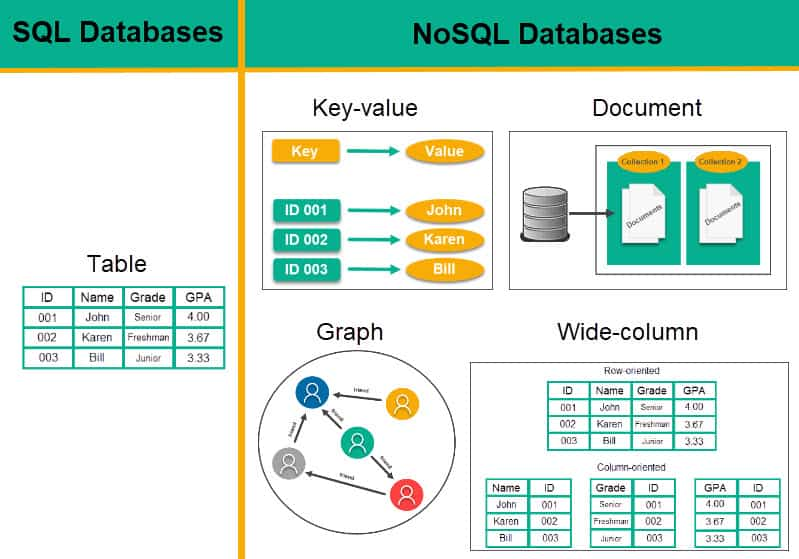
\includegraphics[width=0.8\textwidth]{pics/database-types.jpg}
  \caption{Relational vs. Objektorientiert}
  \cite{database_types}
\end{figure}